\newpage

\chapter{Background}
\label{chap:background}

\section{Decision Trees}

Decision trees are trees where each internal node is associated with an attribute and each of the edges leading out from it are associated with a subset of this attribute's values. The leaf nodes are associated with a class. In order to classify a sample, we start at the root of the tree and follow the edges given by the sample attributes' values. Once we get to a leaf node, we've found the class prediction for this sample.

As an example, let's look at the Titanic Survival dataset (\cite{Titanic}). The picture \ref{fig:titanic-dataset} shows the first 10 samples from the training dataset, where we are trying to predict the value for the Survived field.

\begin{figure}[h]
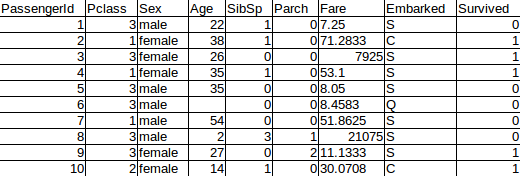
\includegraphics[width=\textwidth]{titanic}
\caption{First ten samples from the Titanic Survival dataset.}
\label{fig:titanic-dataset}
\end{figure}

A possible decision tree is the one given in the figure \ref{fig:titanic-tree}. This tree correctly classifies all the first 10 samples. For instance, since the passanger with Id 1 is male and older than 9.5 years, the decision tree predicts him as someone who did not survive.

\begin{figure}[h]
\centering
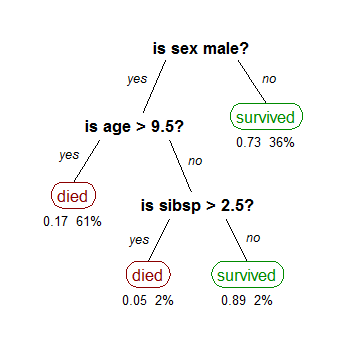
\includegraphics[width=0.75\textwidth]{titanic-tree}
\caption{Possible decision tree for the Titanic Survival dataset.}
\label{fig:titanic-tree}
\end{figure}

The main theme of this dissertation is how to (quickly) create such trees, specially when we have categorical attributes with a large number of values.

\section{Notation}
\label{sec:notation}
We adopt the following notation throughout the dissertation.
Let $S$ be a set of $N$ samples and 
 $C=\{c_1,\ldots,c_k\}$ be the domain of the class label. 
In addition, for an attribute  $A$, we use $A(s)$ to denote the value taken by attribute
$A$ on sample $s$; we use 
  $V=\{ v_1,\ldots,v_n \}$ to denote the set of values
taken by $A$;
$A_{ij}$ to refer to the  number of samples
from class $c_j$ for which  $A$ takes value $v_i$; 
 $N_i$ for the number of samples with value $v_i$ for attribute $A$
and $S_j$ for the number of samples from class $c_j$.
Given a partition $(L, R)$ of the values $V$ of an attribute $A$, we use $S_L$ and $S_R$
to denote the set of samples in $S$ that takes values in $L$ and $R$, respectively, in attribute $A$.
Furthermore, we let $p_j = S_j /N$ and $p_{ij}= Pr[C=c_j | A = v_i]$.
We observe that the estimator of maximum likelihood for $p_{ij} $ is
$A_{ij} / N_i$.  

TODO: definir $S_L$ e $S_R$

\section{Impurity Measures}
Many of the decision tree inducers follow the structure of algorithm \ref{alg:create-tree}.

\begin{algorithm}[tb]
   \caption{CreateTree($S$: set of samples, $List\_A$: list of attributes information, $I$: split impurity measure)}
   \label{alg:create-tree}
\begin{algorithmic}
\IF{$S$ does not meet the stopping criterion}
\FOR{attribute $A$ in $List\_A$}
\STATE $s_A = $ split of $A$ with smallest impurity as measured by $I$
\ENDFOR
\STATE $(L, R) = s_{A^*}$ such that $I(s_{A^*}) \leq I(s_A) $ for any $A$
\STATE CreateTree($L$)
\STATE CreateTree($R$)
\ENDIF
\end{algorithmic}
\end{algorithm}

It is important to note that most impurity calculations on a nominal attribute are done based on what's called a contingency table. It consists of an $n\times k$ matrix where the $ij$-th entry corresponds to the number of samples that have value $i$ and belong to class $k$. We'll assume that every decision tree node has the contingency table pre-calculated for all nominal attributes, which takes $O(N)$ time for each attribute and cannot be avoided\footnote{The only exception is the attribute used to split the parent node, which can be calculated in $O(n\times k)$.}. Therefore, whenever we mention the time complexity for a decision tree constructing algorithm/criterion, this cost will not be mentioned since it does not affect their comparison.

The only thing left is to define what we mean by an impurity measure. \cite{Breiman84} defines a class of imurity measures that are natural in this context.

\begin{definition}
 A function $\phi(p)$ is an impurity measure iff 
 \begin{enumerate}
  \item $\phi: [0, 1] \rightarrow \mathbb{R}_+$;
  \item $\phi$ has continous second derivatires;
  \item $\phi(0) = \phi(1) = 0$;
  \item $\phi(p) = \phi(1-p)$ ($\phi$ is symmetric);
  \item $\phi''(p) < 0$ for $p \in (0, 1)$ ($\phi$ is concave).
 \end{enumerate}
\end{definition}

These impurity measures have the nice property that splitting $V$ into $(L, R)$ always decreases the impurity, as also shown in \cite{Breiman84}.

\begin{theorem}
Given an impurity measure $I$ and any partition of values $V$ into $(L, R)$, we always have
$$I(S) - p_L \cdot I(S_L) - p_R \cdot I(S_R) \geq 0 $$
where $p_L$ and $p_R$ are equal to the ratio of the samples in $L$ and $R$, respectively. Equality happens iff the contingency table in both sides have the same frequency distribution.
\end{theorem}

Another interesting result proven in \cite{Breiman84} is that, when there are only 2 classes, we can find the partition with best impurity in linear time after sorting.

\begin{theorem}
\label{thm:two-class-trick}
Let $I$ be an impurity measure and suppose we only have two classes $c_1$ and $c_2$. The best partition of the values $V$ has the form

$$L = \{v_i : p_{i1} \leq v\}$$
$$R = \{v_i : p_{i1} > v\}$$

for some value $v$.
\end{theorem}

The result above is used by many splitting criteria, as will be mentioned in section \ref{sec:splitting-criteria}.

Now let's present the two most common impurity measures found in the literature. Both can be used to generate binary splits and, as a consequence, binary decision trees.

\begin{definition}
\label{def:Gini}
The Gini Index for a set of samples $S$ is given by 
\begin{equation}
 Gini(S) =  1- \sum_{i=1}^k (p_i)^2 .
\label{eq:gini}
\end{equation}
\end{definition}

\begin{definition}
The Entropy for a set of samples $S$ is given by 
\begin{equation}
 Entropy(S) =  - \sum_{i=1}^k p_i \log p_i
\label{eq:entropy}
\end{equation}
\end{definition}

\section{Splitting Criteria}
\label{sec:splitting-criteria}
In this section we recall some well-known splitting criteria.

First note that, for numeric attributes, all criteria follow the same algorithm to choose the best split: the values are ordered and the valid splits have the form 
$$L = \{v_i : v_i \leq v\}$$
$$R = \{v_i : v_i > v\}$$
for some chosen value $v$. This is because all the acceptable splits should preserve and use the order structure.

The criteria evaluate the impurity of these splits and chooses the one with the smallest impurity. Since we only have to evaluate at a single value $v$ between each pair of consecutive values $v_i$ and $v_{i+1}$, it takes $O(n \log n)$ time. Since this is polynomial and quite fast, its complexity is largely ignored throughout this dissertation.

\subsection{Gini Gain}

The Gini Gain, $\Delta_G$, induced by a binary partition $(L,R)$ of the set of values $V$ is given by 
\begin{equation}
 \Delta_G (L,R) = Gini(S) -
p_L Gini(S_L) - p_R Gini(S_R),
\label{eq:Ginigain}
\end{equation}
where $S_L= \{ s \in S | A(s) \in L \}$, $S_R= \{ s \in S | A(s) \in R \}$,
 $p_L=|S_L| /N $
and $p_R=|S_R| /N$. Therefore, the largest the Gini Gain is, the better the partition.

This criterion generates all $2^n$ binary values' split and the partition with maximum Gini Gain shall be selected.
For the two-class problem this optimal partition can be computed  in $O(n \log n)$ time by using theorem \ref{thm:two-class-trick}. Since we only need to test a single value of $v$ that is between each pair of consecutive values $v_i$, $v_{i+1}$, the time complexity follows.

For problems with more than two classes, however, there is no efficient procedure with theoretical approximation guarantee to compute the Gini Gain in subexponential time in $n$.

\subsection{Twoing}
The Twoing criterion
for a  binary partition $(L,R)$ 
of the set of values $V$ is given by
$$ 0.25 \cdot p_L \cdot p_R  \cdot \left ( \sum_{i=1}^k | p_L^i - p_R^i | \right )^2$$
where

$$ p_L^i= \frac{|\{s \in S_L: s \mbox{ belongs to class } c_i \}|}{ |S_L|} $$
 and 
$$ p_R^i= \frac{|\{s \in S_R: s \mbox{ belongs to class } c_i\} |}{ |S_R|} $$

When the Twoing criterion is used to generate binary decision trees, the binary partition with maximum twoing shall be selected at each node. 

By using theorem \ref{thm:two-class-trick}, the best partition can be found in $O(\min \{ n (k + \log n) 2^k, 2^n \} )$
time by considering all possibilities of partitioning the classes into two superclasses
and applying the Gini Gain criterion on each of them. We shall remark that, for the two-class problem, the Twoing criterion and the Gini Gain compute the same binary partitions.

\subsection{Information Gain}

The Information Gain, $IG$, induced by a binary partition $(L,R)$ 
of the set of values $V$ is given by 
\begin{equation}
 IG(L,R) = Entropy(S) -
p_L Entropy(S_L) - p_R Entropy(S_R),
\label{eq:InformationGain}
\end{equation}
where $S_L= \{ s \in S | A(s) \in L \}$, $S_R= \{ s \in S | A(s) \in R \}$,
 $p_L=|S_L| /N $ and $p_R=|S_R| /N$. Therefore, the largest the Information Gain is, the better the partition.

This criterion works exactly the same as the Gini Gain, but replacing the Gini impurity by the Entropy.

A related criterion is the Gain Ratio, where the Information Gain of an attribute is normalized by that attribute's potential information. This is used as a way of decreasing the bias of the k-ary Information Gain criterion towards attributes with larger number of values. Since we are only interested in binary splits in this dissertation, we will not go into its details.


\subsection{$\chi^2$-criterion}
The $\chi^2$ is a popular criterion that was  used in \cite{Mingers.87}. It is also the first one shown here not based on impurity measures, and it only generates k-ary (instead of binary) splits. Is is mentioned here because of its relation to the framework that will be presented in chapter \ref{chap:framework}.

The $\chi^2$-criterion chooses the attribute $A$ that maximizes
\begin{equation}
\label{eq:chitest}
\sum_{i=1}^n \sum_{j=1}^k \frac{(A_{ij}-E[A_{ij}] )^2}{E[A_{ij}]},
\end{equation}
where $E[A_{ij}]=N_i p_j$.


\subsection{Conditional Inference Trees}
Conditional Inference Trees are actually a framework for creating criteria that are bias-free when it comes to the number of values in an attribute. It was published by \cite{Hothorn:2006:URP} and still is the only known method of obtaining criteria that do not have any bias towards attributes with larger number of values.

It works by first choosing the best attribute to split at the current node and then evaluating all possible binary splits using any given impurity measure, picking the best one found.

To choose the attribute in which to split, first one has to calculate the permutation test's conditional expectation $\mu \in \mathbb{R}^{nk}$ and covariance $\Sigma \in \mathbb{R}^{nk\times nk}$ of every attribute\footnote{Since the formulae are very complicated and won't be used throughout this dissertation, they are ommited. The interested reader can obtain them in the section 3 of  \cite{Hothorn:2006:URP}.}. Then, in order to compare the attributes, we need to calculate the p-value of a univariate test statistics $c$ calculated on $\mu$ and $\Sigma$ of every attribute. The only exact form of doing this comparison is by using the quadratic form $c_{quad}$ (see equation \ref{eq:c_quad}), which follows an asymptotic $\chi^2$ distribution with degrees of freedom given by the rank of $\Sigma$. Since this involves the calculation of a pseudoinverse, which has cubic complexity on the dimension of $\Sigma$, this criterion can be very time consuming.

\begin{equation}
\label{eq:c_quad}
c_{quad}(t, \mu, \Sigma) = (t-\mu)\Sigma^+(t-\mu)\top
\end{equation}

This method, although very complicated and quite slow, is employed by the data mining community when accuracy counts for more than time spent training\footnote{Since this method does not have any bias when choosing which attribute to split, the accuracy of these trees tend to be higher than the trees obtained by biased criteria.}. Thus this criterion will be used in our experiments in chapter \ref{chap:experiments-datasets} to compare the different accuracies obtained when changing the splitting criterion used to choose the attribute's values split.

\section{Heuristics for Splitting Decision Tree Nodes}
As seen in the previous section, calculating the optimal binary split takes exponential time in the number of values or classes. Therefore many heuristics were created to construct decision trees in this situation. The most used ones are listed below. All of them work with any impurity measure (e.g.: Gini or Entropy), but some of them work best with just one of them. When this is the case, it will be mentioned.

\subsection{Hypercube Cover}

The Hypercube cover criterion works exactly the same as the Twoing criterion except when it comes to the split impurity calculation. Instead of calculating the impurity based on the two superclasses, Hypercube Cover calculates it using the original $k$ classes. This guarantees, for instance, that the split impurity, when measured with respect to the original classes, is never worse than that of Twoing. This method was first suggested in \cite{icml2018}, together with its approximation guarantee of 2 for both the Gini and Entropy impurities.


%\subsection{SLIQ and SLIQ-ext}
%SLIQ was presented in \cite{mehta1996sliq} and it's a very simple greedy heuristic. Given an attribute, one starts with all the values going to the left split, and none on the right split. We then choose a value to go from the left to the right split. This value is the one that, when changing from the left to the right sides, decreases the impurity (increases the impurity gain) the most. This is repeated until there is no way of moving a value from the left to the right and decreasing the impurity.
%
%SLIQ-ext is a simple extension, where we keep changing values from the left to the right until the left side is empty (that is, we move from the left to the right even if that increases the impurity). Once again the value to move is chosen in a greedy fashion. SLIQ-ext returns the values' split seen that had the lowest impurity.


\subsection{PC and PC-ext}
These heuristics are based on the Principal Component of the contingency table and were presented in \cite{journals/datamine/CoppersmithHH99}.
They are based on a theorem that states that the optimal partition of values can be found by separating the class probability vectors by a hyperplane.

\begin{theorem}{Hyperplanes lemma}
 Let $I$ be an impurity measure. If $(L, R)$ is an optimal partition for the values $V$ then there is a vector $d \in \mathbb{R}^k$ such that
 
 $$d\cdot\pi(v) < 0, \forall v \in L$$
 $$d\cdot\pi(v) > 0, \forall v \in R$$
 
 where $\pi(v) = v / \lVert v \rVert_1$.
\end{theorem}


In other words, in order to find the optimal partition we just need to choose the right hyperplane. This motivates the PC criterion, which look at the hyperplanes in $\mathbb{R}^k$ whose normal vector is the principal direction of the attribute's contingency table.

In more details, one first calculates the class probability distribution of every value, which is done by normalizing the contingency table rows to measure 1 in the sum norm. Then the values are grouped into ``supervalues'' where all values in the same supervalue have the same class probability distribution. Now the first principal component of these sypervalues' contingency table is calculated. One then calculates the inner product of each class probability vector of the supervalues  with the principal component and sort the supervalues by it. Denote by $v_1,\ldots,v_{n^*}$ the $n^*$ supervalues sorted in this manner and denote by $p$ the first principal component. We then calculate the impurity gain of all the supervalues' splits of the form

$$L = \{v_i | v_i \cdot p \leq t\}$$
$$R = \{v_i | v_i \cdot p > t\}$$

where $t$ is a chosen threshold. Once we find the supervalues split with the largest impurity gain among them, we choose it and translate the supervalues into original values to obtain a valid partition.

PC-ext is a simple extension of this algorithm, where instead of only testing the supervalues splits given by the equations above, we also test the splits given by  exchanging the last supervalue on the left with the first supervalue on the right (where first and last are given by the order after calculating the inner product).

These procedures require $O(k^3)$ operations to find the principal component and $O(n)$ impurity calculations and inner products in the class probability space.

\subsection{Largest Class Alone}

This is a heuristic that, when using the Gini impurity, has an approximation guarantee of 2 compared with the optimal partition found by Gini Gain.

First one calculates the most frequent class and group the other classes in a single superclass. One then applies the Gini Gain criterion on this two-class problem. Since calculating the class frequencies can be done using the contingency table, this heuristic takes $O(N + n k + n \log n)$ time in total.

It can also be used with the Information Gain impurity, instead of Gini Gain, but its approximation guarantee increases to 3. These bounds are all proved in \cite{icml2018}.

\subsection{List Scheduling}

Similarly to the Largest Alone heuristic, List Scheduling is a criterion that has an approximation guarantee of 2 for the Informatio Gain criterion when using the Entropy impurity.

First one calculates the frequency of every class. Then, one groups the classes into 2 superclasses as balanced as possible in terms of number of samples. Lastly the Information Gain criterion is applied on this two-class problem.

Since finding the most balanced partition is NP-complete, we settle for a List Scheduling algorithm to find a partition with a 4/3-approximation guarantee to the optimal one. Since calculating the class frequencies can be done using the contingency table and the List Scheduling algorithm is linear in the number of classes, this takes $O(N + n k + n \log n)$ time in total. Note that, since we are not necessarily using the most balanced partition, there is no guarantee that we will be within a factor of 2 of the optimal impurity.

This criterion is based on a result proved in \cite{icml2018} which states that, for the entropy impurity, the best form of grouping classes into superclasses is by balancing them the most.